\section{Auswertung}

\subsection*{Vorbemerkungen}

Sofern nicht anders angegeben, berechnen wir die Fehler zusammengesetzter Werte anhand der standardmäßigen Gauß'schen Fehlerfortpflanzung. Die $\sigma$-Abweichung zweier fehlerbehafteter Werte $x \pm \Delta x$ und $y \pm \Delta y$ berechnen wir anhand der Formel
\begin{align}
  \sigma = \frac{\qty|x - y|}{\sqrt{\Delta x^2 + \Delta y^2}}.
\end{align}

Für eine Anzahl an Ereignissen $N$ berechnet sich der Fehler gemäß $\Delta N = \sqrt{N}$. Zur Fehlerangabe für Zählraten $n = \flatfrac{N}{t}$ leiten wir daraus die Formel
\begin{align}
  \Delta n = \frac{\Delta N}{t}= \frac{\sqrt{N}}{t} = \frac{\sqrt{nt}}{t} = \sqrt{\frac{n}{t}}
\end{align}
ab.

\subsection{Röntgenspektrum mit LiF-Kristall}

\abbref{fig:spektrum_lif_komplett} zeigt das Röntgenspektrums, welches wir mit der Drehkristallmethode mit einem LiF-Kristall im Winkelbereich von $3\si{\degree}$ bis $22\si{\degree}$ aufgezeichnet haben. Bereits hier ist zu erkennen, dass wir ab einem Winkel von etwa $5\si{\degree}$ beginnen, Bremsstrahlung zu detektieren.

\begin{figure}[H]
  \centering
  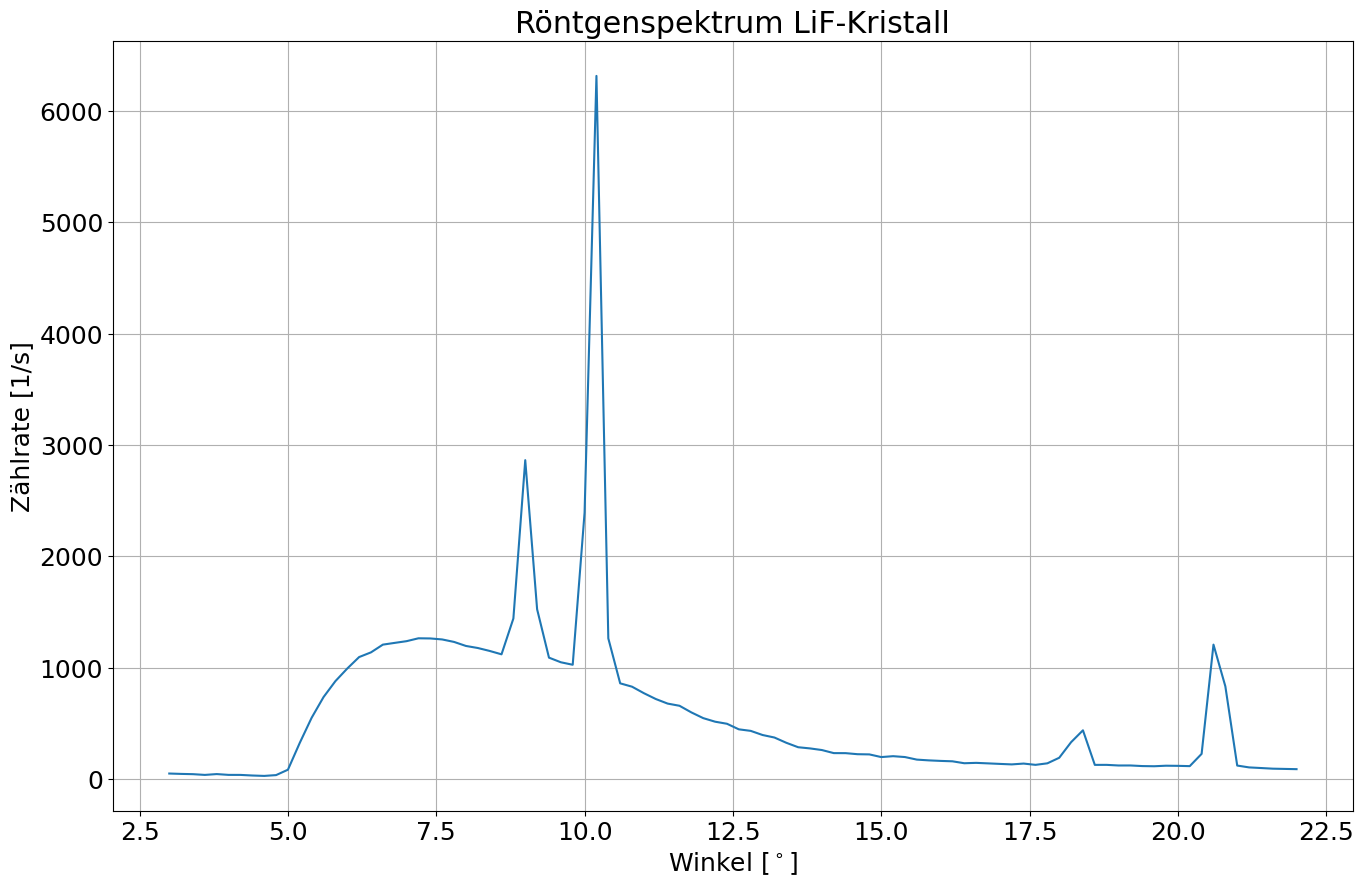
\includegraphics[width=.9\textwidth]{files/plots/spektrum_lif_komplett.png}
  \caption{Röntgenspektrum mit LiF-Kristall}
  \label{fig:spektrum_lif_komplett}
\end{figure}

Um den Winkel und die zugehörige Grenzwellenlänge genauer zu bestimmen, betrachten wir den nahezu linearen Bereich des Spektrums am kurzwelligen Ende und fitten an dieses eine lineare Funktion der Form $f(x;a,b) = ax + b$, wie in \abbref{fig:spektrum_lif_linear_fit} zu sehen.

\begin{figure}[H]
  \centering
  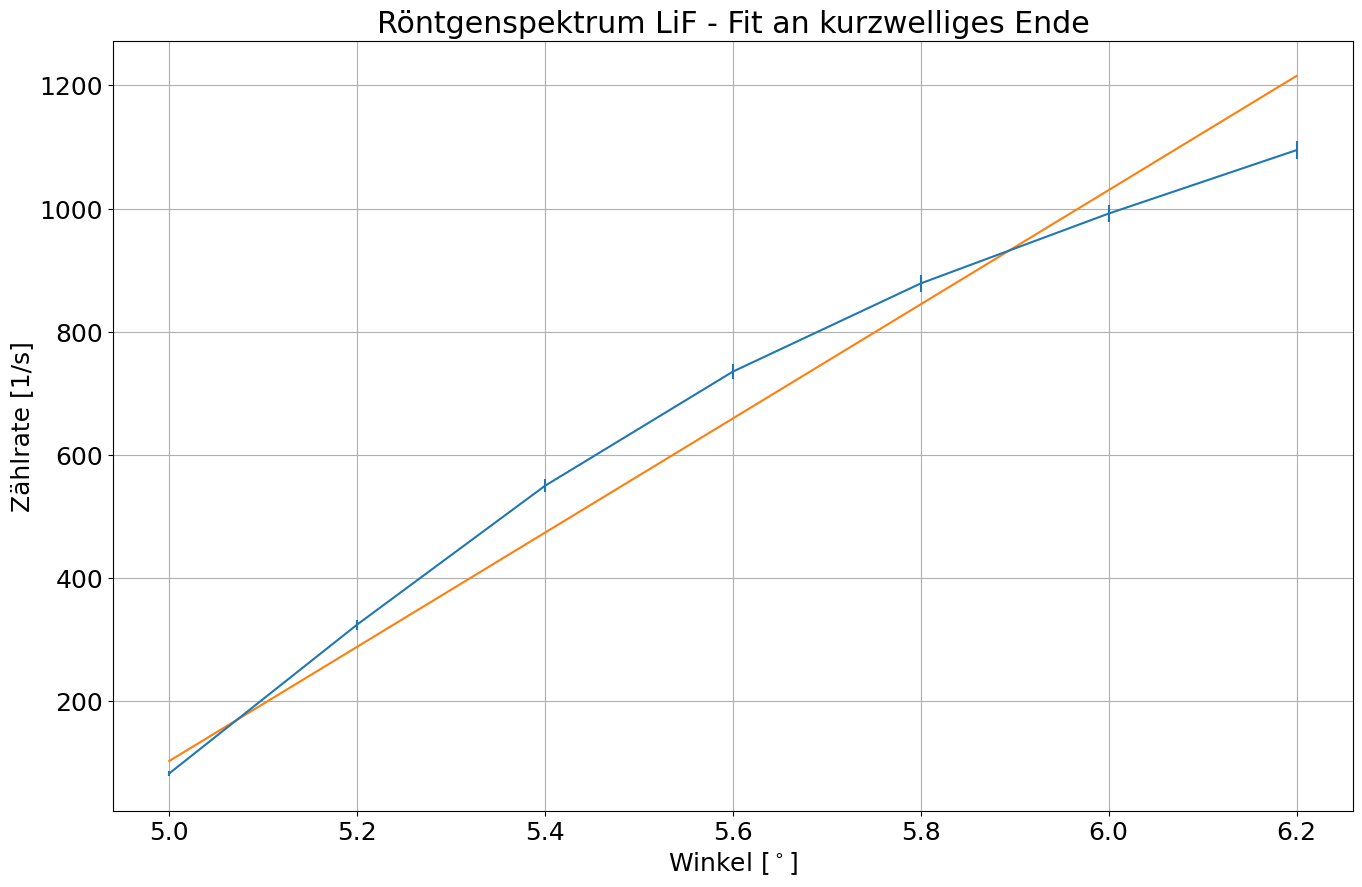
\includegraphics[width=.9\textwidth]{files/plots/spektrum_lif_linear_fit.png}
  \caption{spektrumliflinearfit}
  \label{fig:spektrum_lif_linear_fit}
\end{figure}

Für die optimierten Parameter erhalten wir die Werte
\begin{align}
  a = 926.94 \pm 56.62 \si{\per\second\per\degree},\quad
  b = -4531.53 \pm 297.50 \si{\per\second}.
\end{align}
Mit diesen berechnen wir den Winkel, ab dem die Bremsstrahlung einsetzt, als Nullstelle der linearen Funktion nach
\begin{align}
  \vartheta_{0,1. Ord} = -\frac{b}{a} = 4.9 \pm 0.5 \si{\degree}.
\end{align}

Mithilfe des Bragg'schen Gesetzes \eqref{eq:bragg} können wir daraus nach
\begin{align}
  \lambda = \frac{2d\sin(\vartheta)}{n}
\end{align}
die entsprechende Grenzwellenlänge berechnen. Da es sich hierbei um den Einsatz des Spektrums erster Ordnung handelt, setzen wir $n = 1$. Den Netzabstand $d$ des LiF-Kristalls entnehmen wir aus der Praktikumsanleitung als $d = 201.4\si{\pico\meter}$. Damit erhalten wir für die Grenzwellenlänge einen Wert von
\begin{align}
  \lambda_{Grenz} = (34.33 \pm 3.08) \si{\pico\meter}.
\end{align}

Setzen wir nun in \eqref{eq:grenzfreq} diese Grenzwellenlänge, die Spannung $U = 35\si{\kilo\volt}$ ein und stellen diese nach dem Plank'schen Wirkungsquantum $h$ um, so erhalten wir für dieses einen Wert von
\begin{align}
  h = (6.4 \pm 0.6) \cdot 10^{-34} \si{\joule\second}.
\end{align}

Die Grenzwellenlänge $\lambda_{grenz}$ können wir weitergehend einsetzen, um den Winkel zu bestimmen, ab dem das Spektrum zweiter Ordnung einsetzt. Dazu stellen wir \eqref{eq:bragg} nach $\vartheta$ um, und setzen $n = 2$. Wir erhalten damit einen Winkel von
\begin{align}
  \vartheta_{0,2. Ord} = (9.813 \pm 0.016)\si{\degree}.
\end{align}